\documentclass{beamer}

\usepackage{graphicx} % Required for inserting images
\usepackage{xeCJK}
\usepackage{amsmath, amssymb, amsthm, amsfonts}
\usepackage{unicode-math}
\usepackage{algorithm}
\usepackage{algpseudocode}
\usepackage{multirow, multicol}
\usepackage{siunitx}
\usepackage{animate}
\usepackage[labelformat=simple]{subcaption}
\usepackage{comment}

%,algorithm2e,float
\usepackage{hyperref}

\usepackage{biblatex}
\addbibresource{ref.bib}

% Define operator
\DeclareMathOperator*{\argmax}{argmax}
\newcommand{\algorithmicbreak}{\textbf{break}}

%theme settings

%\usetheme{Madrid}
%\usetheme{Ilmenau}
%\usetheme{Berlin}
%\usetheme{Darmstadt}
\usetheme{Frankfurt}
%\usetheme{Ilmenau}
%\usetheme{Singapore}

\usecolortheme{default}
\definecolor{UQmain}{rgb}{0.4,0.4,0.8}
\setbeamercolor*{palette primary}{bg=UQmain, fg=white}
\setbeamercolor*{palette secondary}{bg=white, fg=UQmain}
\setbeamercolor*{palette tertiary}{bg=UQmain, fg=white}
\setbeamercolor*{palette quaternary}{bg=UQmain, fg=white}
\AtBeginEnvironment{thm}{%
    \setbeamercolor{block body}{bg=white, fg=black}
    \setbeamercolor{block title}{bg=UQmain, fg=white}}


\setCJKmainfont{AR PL UKai TW}
% 這兩行一定要加，中文才能自動換行
\XeTeXlinebreaklocale "zh" 
\XeTeXlinebreakskip = 0pt plus 1pt



\title{Trend Analysis and Change Points Detection}
\author[SHAN-CHI, WU]{SHAN-CHI WU \inst{}}
%\advisor{Chu-Lan Michael Kao}
\institute[]{\inst{} Institute of Statistical Science, Academia Sinica, Taiwan}
\date{October 9, 2024}%\today

\begin{document}

\begin{frame}
    \maketitle
\end{frame}

\begin{frame}{Outline}
    \tableofcontents
\end{frame}


\section[Intro.]{Introduction}

\begin{frame}{Introduction}
    \begin{itemize}
        \item \textbf{Trend Analysis} is a statistical method used to assess trends or patterns in a dataset. %This analysis helps identify the long-term changes in the data. Trend analysis typically involves detecting trends, periodic variations, and other patterns in the data to predict future developments.
        \bigskip

        \item \textbf{Change Point Detection (CPD)} is an analytical method used to identify change points or breakpoints in time series data. %Change points represent moments or periods in a time series where the structure or statistical characteristics suddenly change. Change point detection aims to identify these changes to understand the dynamic variations in the data better.
        \bigskip
        
        \item This slide will present several methodologies for identifying change points, encompassing mean, slope, and variance changes. 
        \bigskip
        
        \item Additionally, we will examine various approaches, ranging from traditional statistical perspectives to contemporary machine learning and deep learning frameworks. 
    \end{itemize}
\end{frame}

\begin{frame}{Trend analysis}
    \begin{itemize}
        \item \textbf{Decomposition of Time Series:}
            \begin{align*}
                Y_t = T_t + S_t + \varepsilon_t, \quad E\varepsilon_t=0 \\
                S_{t+d}=S_t, \quad \sum_{t=1}^d S_t=0
            \end{align*}
        $Y_t$ : observed time series data; $T_t$ : long-term trend;\\ 
        $S_t$ : seasonal patterns; $\varepsilon_t$ : irregular patterns.
        
        \item \textbf{Trend analysis} often refers to techniques for extracting an underlying pattern of behavior in a time series, which would otherwise be partly or nearly completely hidden by noise.
        
        \item If the trend can be assumed linear, a trend analysis can be performed within a formal regression analysis. Otherwise, trend testing can be done using non-parametric methods, e.g., the Mann-Kendall test. %Smoothing can also be used to test and visualize non-linear trends. 
    \end{itemize}
\end{frame}


\begin{frame}{Decomposition of Time Series}
    \begin{figure}
        \centering
        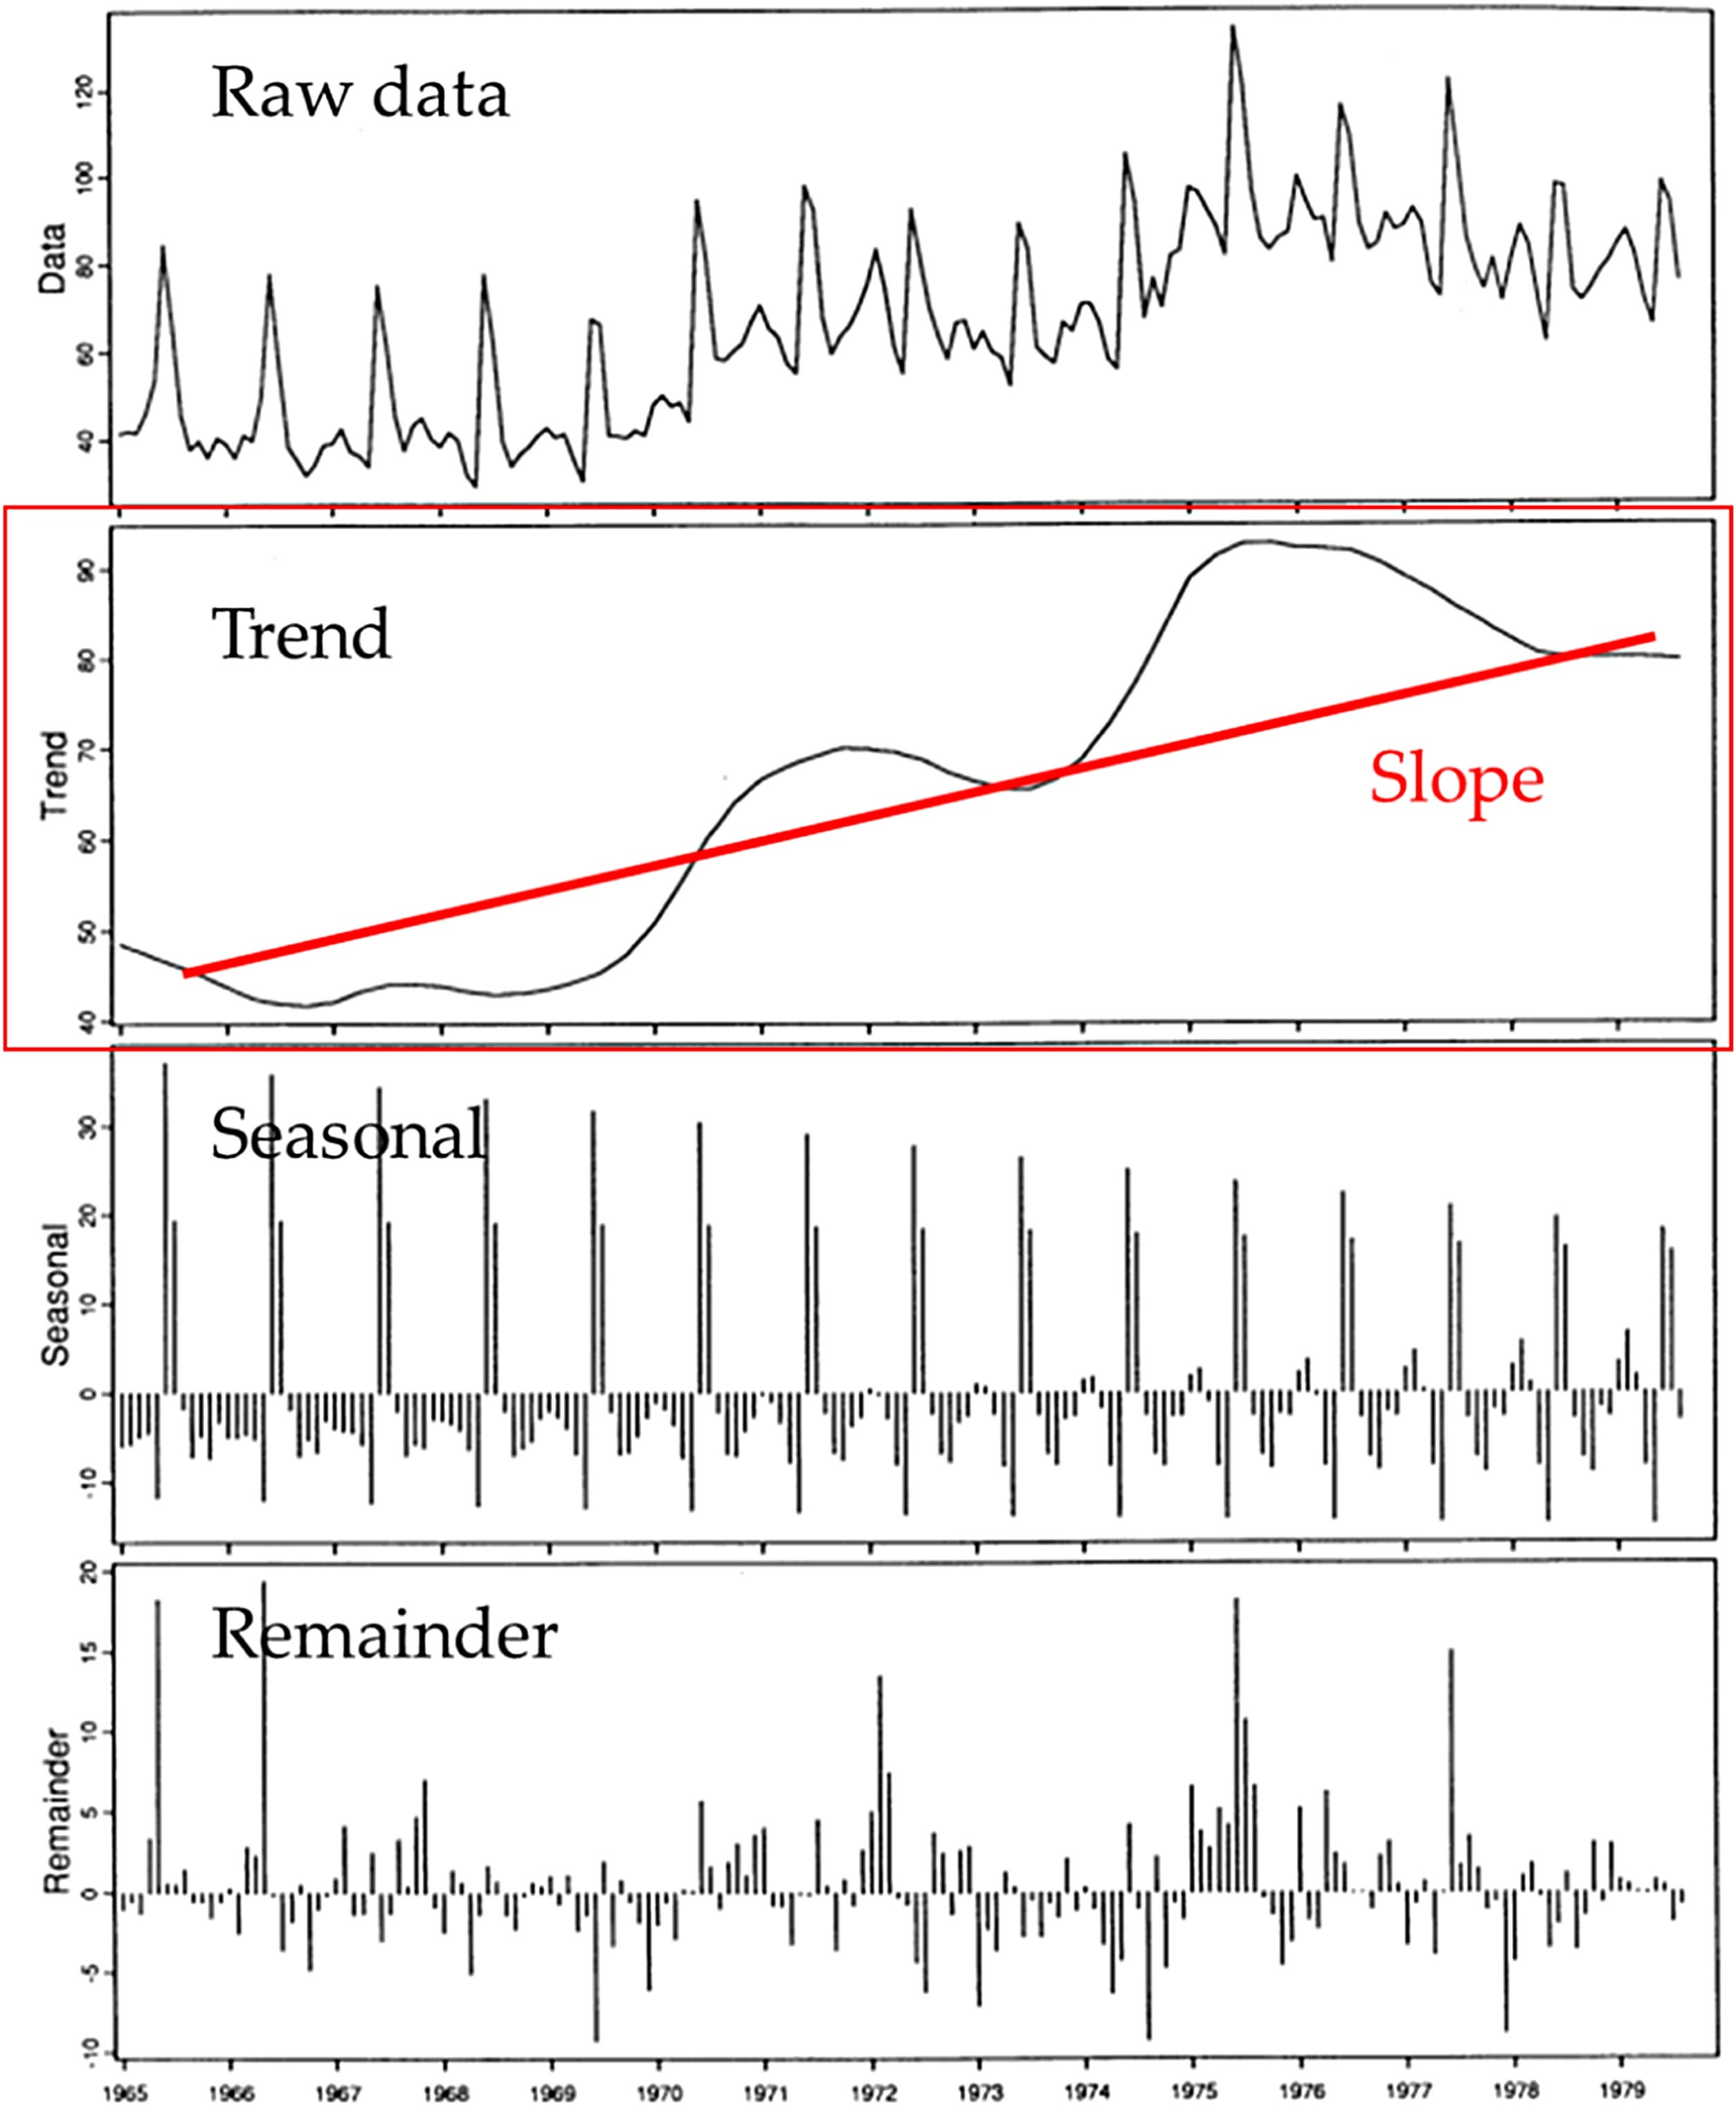
\includegraphics[width=5.5cm]{figure/TSD.jpg}
        \caption{Example of time series decomposition (Song et al. 2021)}
        \label{fig:TSD}
    \end{figure}
\end{frame}



\section[Trend Analysis]{Trend Analysis}

\subsection{Interrupt Time Series}

\begin{frame}{Interrupt Time Series}
    \begin{itemize}
        \item \textbf{Interrupt Time Series (ITS)} refers to sudden events or interruptions in time series data. \\ 
        A minimum of three variables are required for an ITS analysis: %Such interruptions can impact the analysis and modeling of time series data, so they must be considered when conducting relevant analyses.

        \begin{enumerate}
            \item ⁠$T$: the time elapsed since the start of the study in
            
            \item ⁠$X_t$: a dummy variable that indicates the pre-intervention period (coded 0) or the post-intervention period (coded 1)
            
            \item $Y_t$ : the outcome at time $t$
        \end{enumerate}

        \item In standard ITS analyses, the following segmented regression model is used:
    \begin{align*}
        Y_t = \beta_0 + \beta_1 T + \beta_2 X_t+ \beta_3 T X_t , 
    \end{align*}
        which represents the impact model of level and slope change.
        
        \item The level change and the slope change can be specified by excluding the terms $\beta_3 T X_t$ or $\beta_2 X_t$, respectively
    \end{itemize}
\end{frame}

\begin{frame}{Interrupt Time Series}
    \begin{figure}
        \centering
        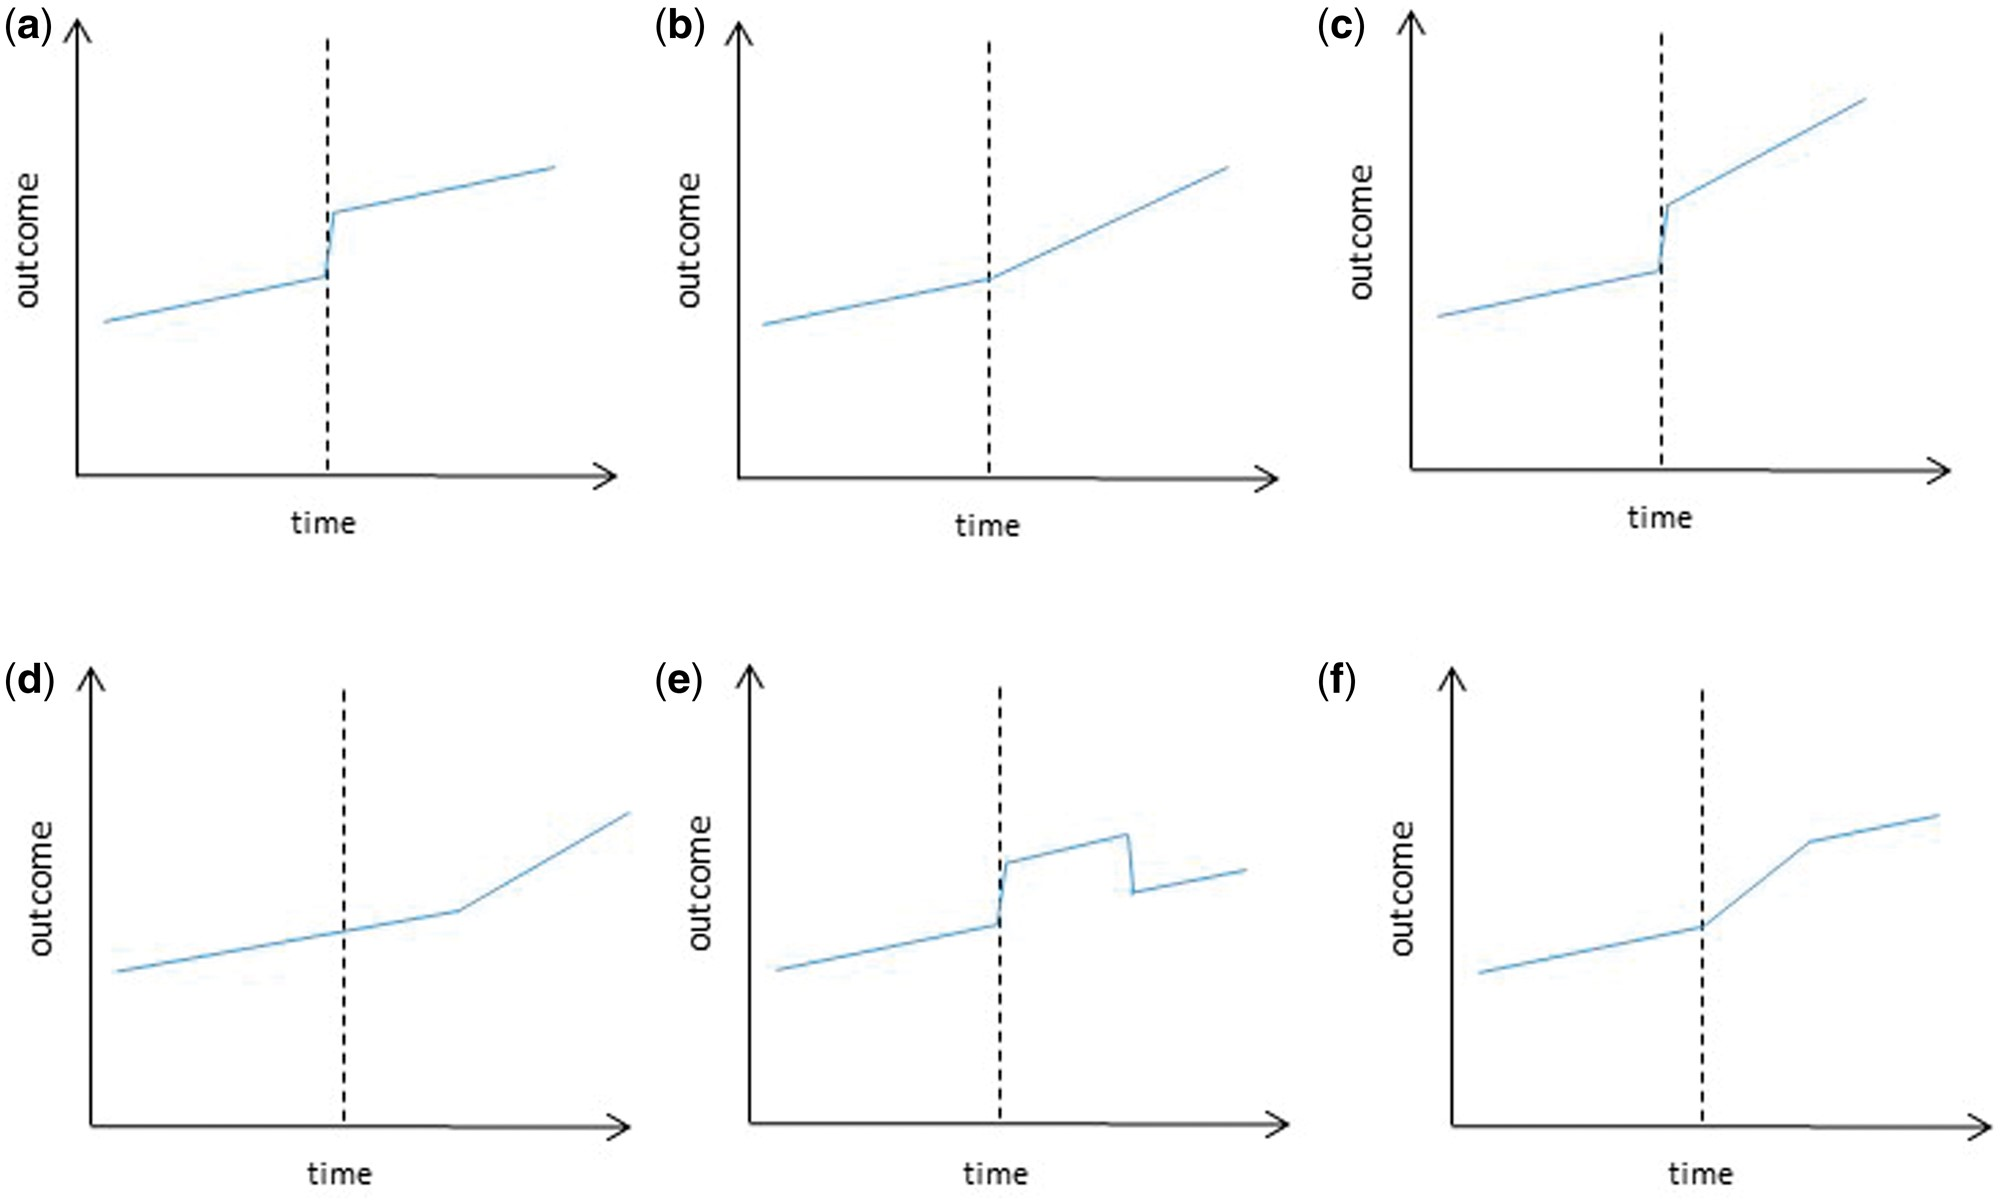
\includegraphics[width=10cm]{figure/ITS.jpeg}
        \caption{Example of interrupt time series (Bernal et al. 2017)}
        \label{fig:ITS}
    \end{figure}
\end{frame}

\begin{frame}{Interrupt Time Series}
    \begin{itemize}
        \item There are several issues with time series data that may need to be addressed to improve the robustness of the analysis
        \begin{multicols}{2}
            \begin{enumerate}
                \item Seasonality
                \item Time-varying confounders
                \item Over-dispersion
                \item Autocorrelation
            \end{enumerate}
        \end{multicols}
    \end{itemize}

    \begin{figure}
	\begin{subfigure}{.31\textwidth}
		\centering
		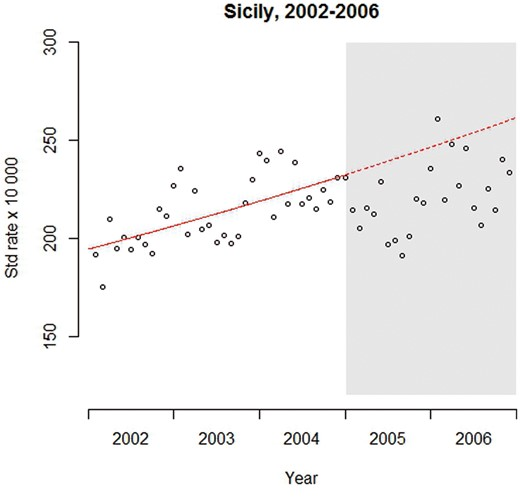
\includegraphics[width=\textwidth]{figure/ITS_1.jpeg}
		\caption{Regression}\label{fig:ITS_1}
	\end{subfigure}
    \begin{subfigure}{.31\textwidth}
		\centering
		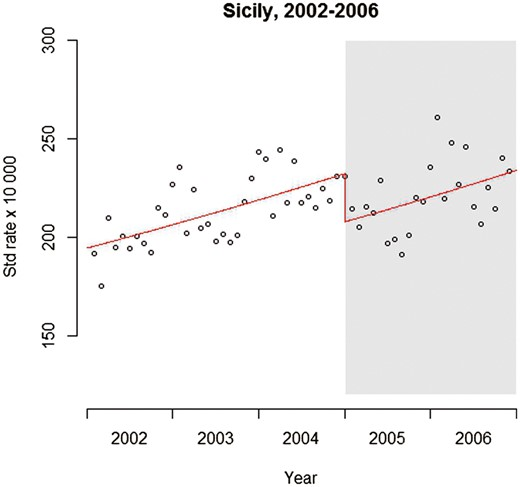
\includegraphics[width=\textwidth]{figure/ITS_2.jpeg}
		\caption{Add level change}\label{fig:ITS_2}
	\end{subfigure}
    \begin{subfigure}{.31\textwidth}
		\centering
		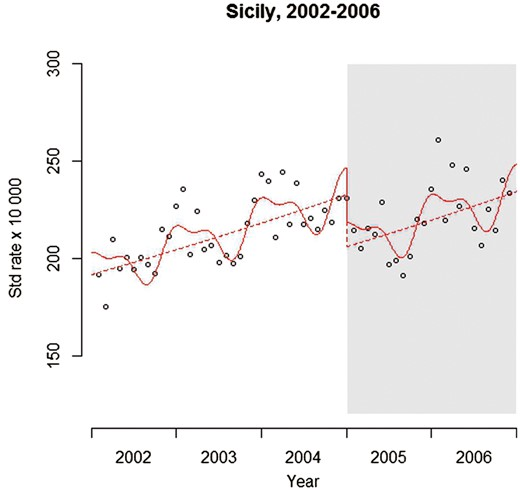
\includegraphics[width=\textwidth]{figure/ITS_3.jpeg}
		\caption{Add seasonality}\label{fig:ITS_3}
	\end{subfigure}
    \caption[]{Fitting result of interrupt time series (Bernal et al. 2017)}\label{fig:ITS_eg}
    \end{figure}
\end{frame}

\subsection{Two-phase regression}

\begin{frame}{Two-phase regression}
    \begin{itemize}
        \item If we don't know where the change point is, we can apply the two-phase regression model (Reeves, 2007)
        \begin{align*}
            Y_t =
            \begin{cases}
                \mu_1 + \beta_1 t + \varepsilon_t, & 1 \leq t \leq c \\
                \mu_2 + \beta_2 t + \varepsilon_t, & c+1 \leq t \leq n,
            \end{cases}
        \end{align*}
        which allows both step-type $\mu_1 \neq \mu_2$ and trend-type $\beta_1 \neq \beta_2$ change points. The null and alternative hypotheses are
        \begin{align*}
            H_0&: \mu_1 = \mu_2 \text{ and } \beta_1 = \beta_2 \\
            H_A&: \mu_1 \neq \mu_2 \text{ and/or } \beta_1 \neq \beta_2
        \end{align*}
    \end{itemize}
\end{frame}

\begin{frame}{Two-phase regression}
    \begin{itemize}
        \item Fix $c$, then $H_0$ could be tested by simply using the standard $F$-test for model reduction:
        \begin{align*}
            F_c = \frac{(\text{SSE}_0-\text{SSE}_A)/2}{\text{SSE}_A/(n-4)} \sim F_{2,n-4},
        \end{align*}
        where $\text{SSE}_0$ and $\text{SSE}_A$ are the sum of squared errors computed under $H_0$ and $H_A$ (with a change point at $c$), respectively.
        \bigskip
        
        \item Large $F_c$ values suggest $H_A$ with a change point at time $c$. Since $c$ is unknown, we use
        \begin{align*}
            F_{\text{max}} = \max_{1\leq c<n} F_c
        \end{align*}
        as the test statistic. 
    \end{itemize}
\end{frame}

\section[Mean CPD]{Mean Change Point Detection}

\begin{frame}{Change Point Detection}
    \begin{itemize}
        \item \textbf{Change point detection (CPD)} is the task of finding changes in the underlying model of a signal or time series. \\ 
        For example, climate change detection, speech recognition, human activity analysis, etc. 
        \bigskip

        \item Define a $\varepsilon$-real-time algorithm that needs at least $\varepsilon$ data samples in the new batch of data to be able to find change points
        \bigskip
        
        \item \textbf{online methods}: aim to detect changes as soon as they occur in a real-time setting (anomaly detection, $\varepsilon \rightarrow 0$)
        \bigskip
        
        \item \textbf{offline methods}: retrospectively detect changes when all samples are received (signal segmentation, $\varepsilon \rightarrow \infty$)
    \end{itemize}
\end{frame}

\begin{frame}{Change Point Detection}
    The state change is related to the change points (change in mean).
    \begin{figure}
        \centering
        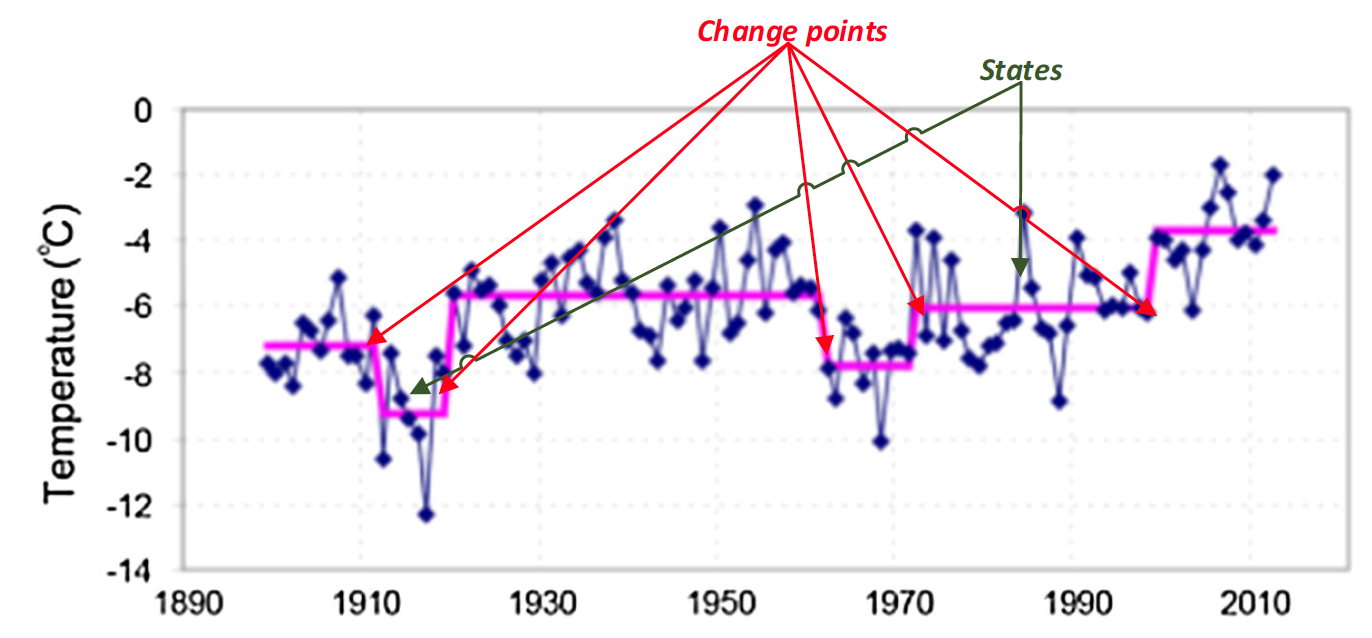
\includegraphics[width=10cm]{figure/CP_example.png}
        \caption{Sample time series and change points (horizontal lines indicate separate states) (Samaneh et al. 2017)}
        \label{fig:CPD}
    \end{figure}
\end{frame}

\begin{frame}{Change Point Detection}
    \begin{itemize}
        \item The following provides an overview of the basic algorithms commonly applied to the CPD problem.
        \bigskip

        \item \textbf{Supervised method} are ML algorithms that learn a mapping from input data to a target attribute of the data, usually a class label.\\
        \smallskip
        If the number of states is specified, the change point detection algorithm is trained to find each state boundary.
        \bigskip
        
        \item \textbf{Unsupervised method} are typically used to discover patterns in unlabeled data. They can be used to find change points based on statistical features of the data.\\
        \smallskip
        It is more attractive because it may handle various situations without requiring prior training for each situation. 
    \end{itemize}
\end{frame}

\subsection{Supervised method}

\begin{frame}{Supervised method}
    \begin{figure}
        \centering
        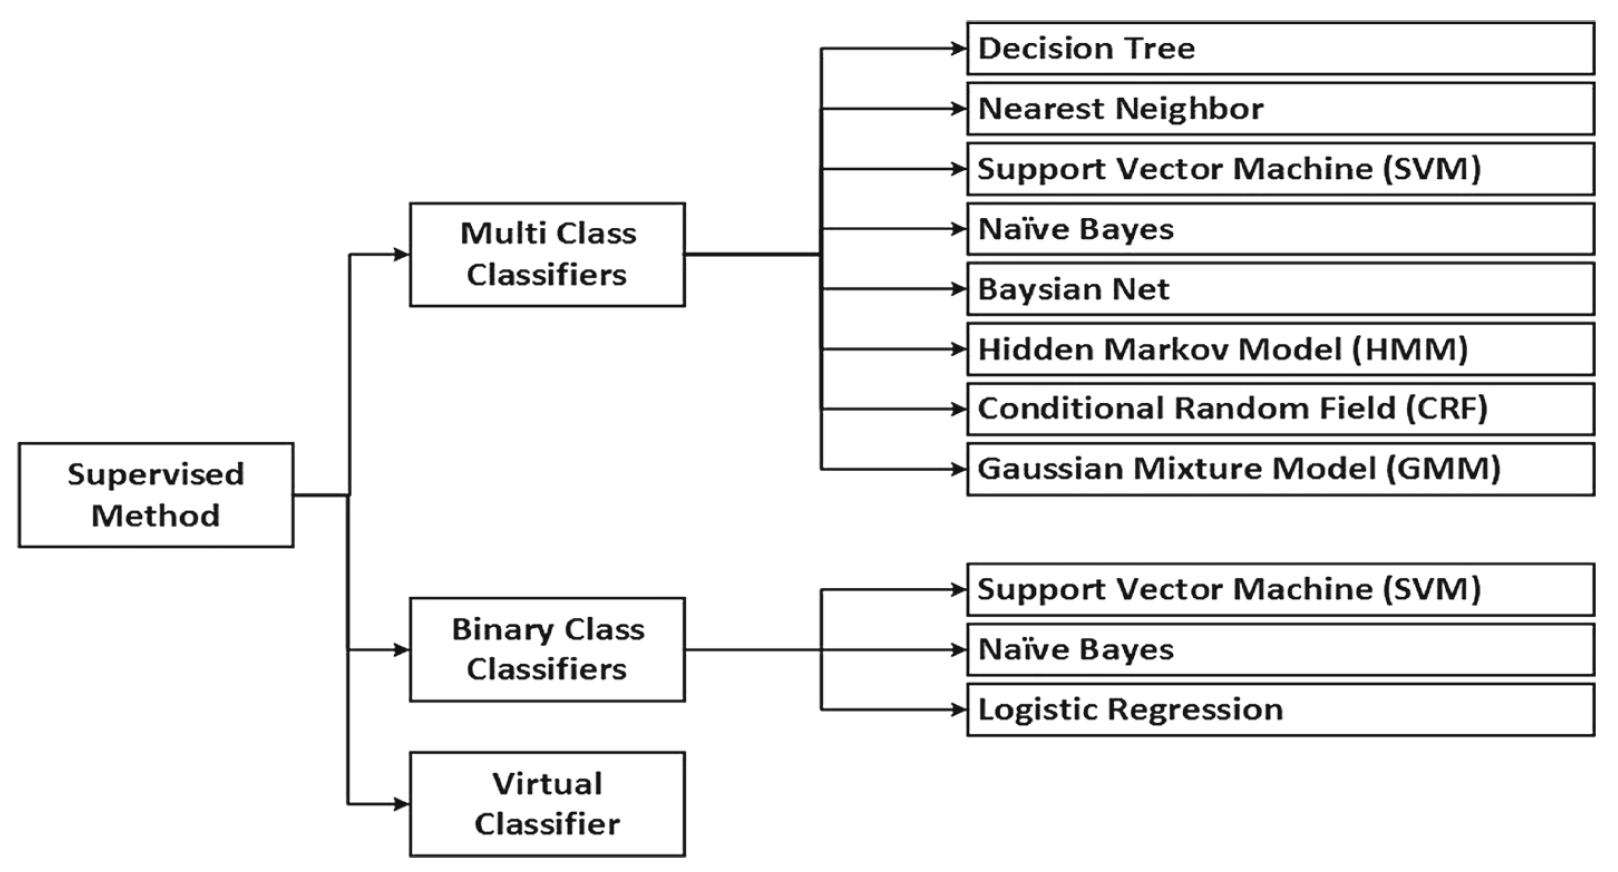
\includegraphics[width=10cm]{figure/SM.png}
        \caption{Supervised methods for CPD (Samaneh et al. 2017)}
        \label{fig:SM}
    \end{figure}
\end{frame}

\begin{frame}{Supervised method - Virtual classifier}
    \begin{itemize}
        \item Attach a hypothetical label $+1$ to each sample of $X_A$, and $−1$ to each sample of $X_B$. Then, train a classifier with the supervised method

        \item If two data sets have differences, they should be correctly classified by the classifier. Thus a high classification accuracy $p$ indicates a difference between $X_A$ and $X_B$
    \end{itemize}

    \begin{figure}
        \centering
        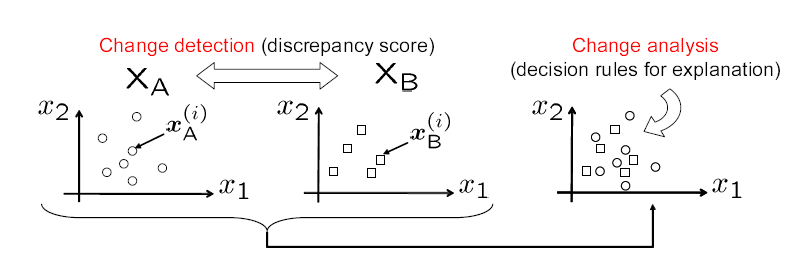
\includegraphics[width=10cm]{figure/VC.png}
        \caption{virtual classifier approach (Hido et al. 2008)}
        \label{fig:VC}
    \end{figure}
\end{frame}


\subsection{Unsupervised method}

\begin{frame}{Unsupervised method}
    \begin{figure}
        \centering
        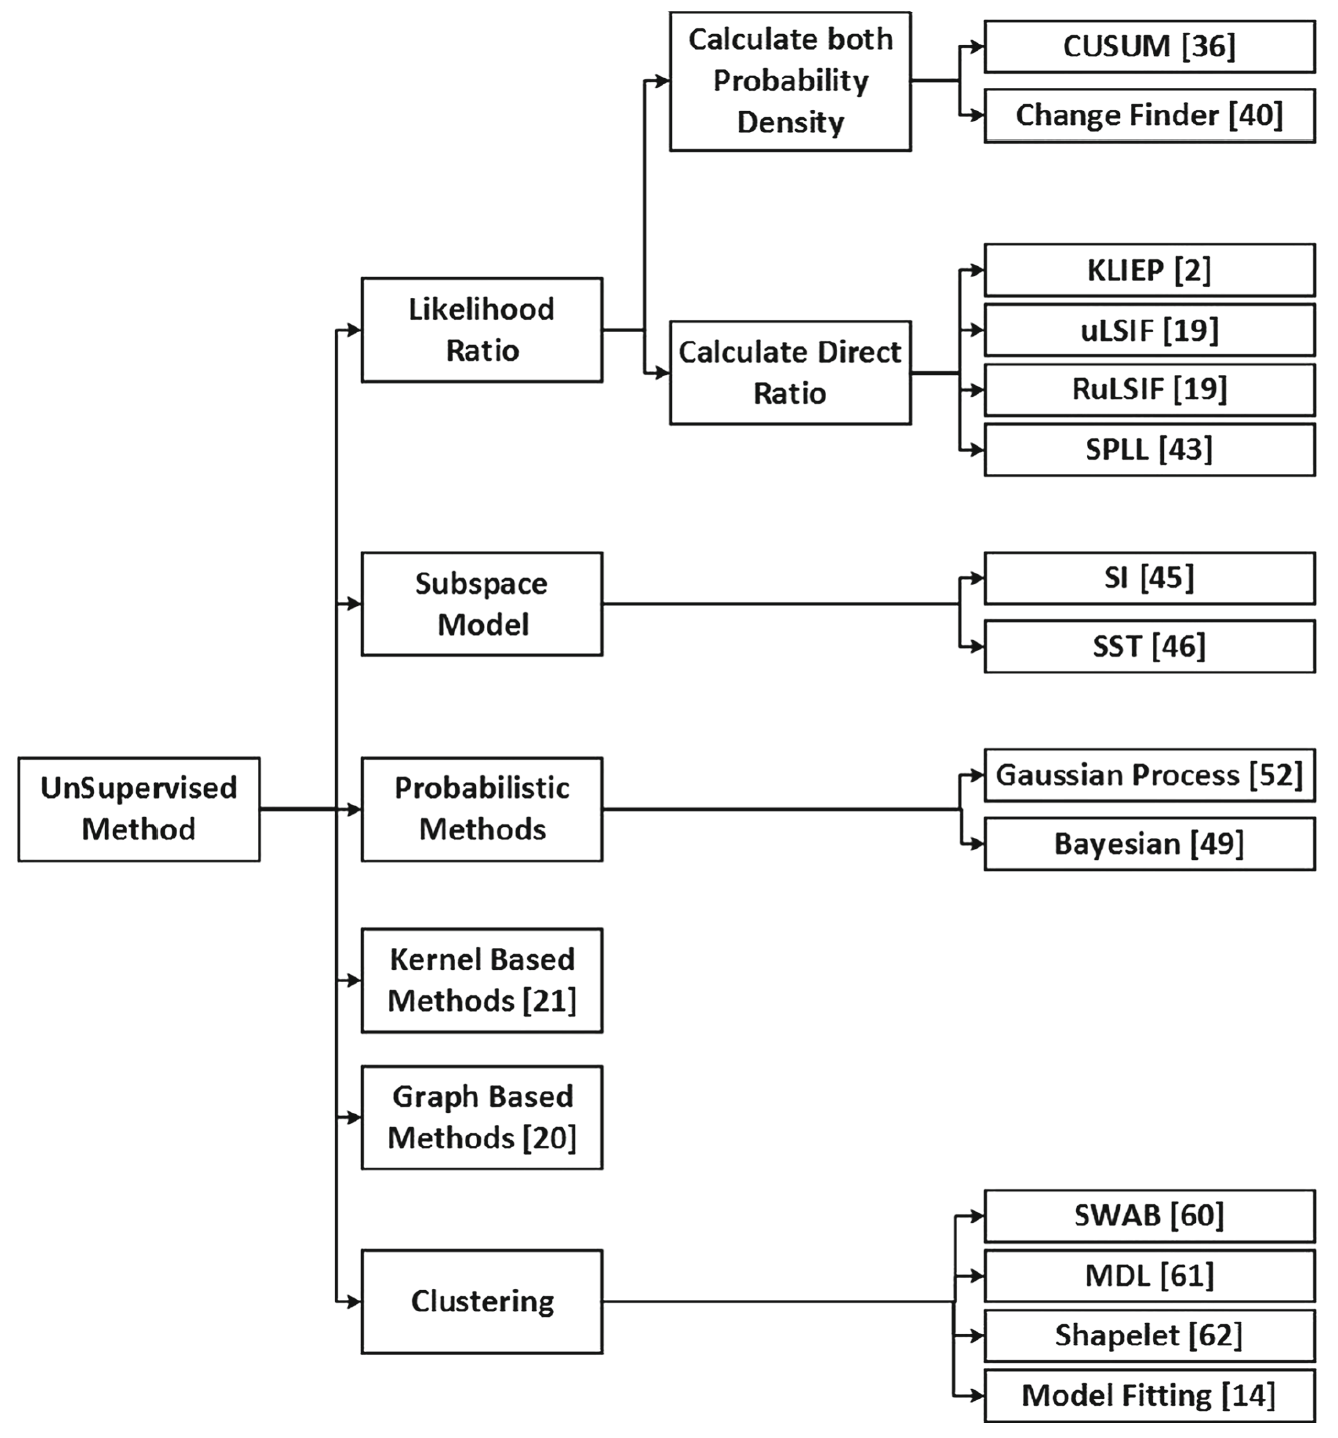
\includegraphics[width=6cm]{figure/USM.png}
        \caption{Unsupervised methods for CPD (Samaneh et al. 2017)}
        \label{fig:USM}
    \end{figure}
\end{frame}

\begin{frame}[allowframebreaks]{Unsupervised methods}
    \begin{itemize}
        \item \textbf{Likelihood ratio methods:} \\ 
        Based on the observation, the probability density of two consecutive intervals is the same if they belong to the same state. 
        \bigskip
        
        \item \textbf{Subspace modeling:} \\
        Represents a time series using state spaces, thus detecting change points by predicting the state space parameters. 
        \bigskip
        \item \textbf{Probabilistic methods:} \\ 
        Estimate probability distributions of the new interval based on the data observed since the previous candidate change point. 
        \bigskip \framebreak
        
        \item \textbf{Kernel-based methods:} \\
        Map observations to a higher-dimensional feature space and detect change points by comparing the homogeneity of each subsequence. 
        \bigskip
        
        \item \textbf{Graph-based technique:} \\
        A newly introduced method that represents time series observations as a graph and applies statistical tests to detect change points based on this representation. 
        \bigskip
        
        \item \textbf{Clustering methods:} 
        Group time series data into their respective states and find changes by identifying differences between features of the states.
    \end{itemize}
\end{frame}

\begin{frame}{Unsupervised methods - Subspace model}
    \begin{itemize}
        \item The Singular Spectrum Transformation (SST) is based on a state-space model. Define a trajectory matrix based on an explained Hankel matrix for each window:
        \begin{align*}
        X=
        \begin{pmatrix}
        y_1    & y_2     & \cdots & y_K     \\
        y_2    & y_3     & \cdots & y_{K+1} \\
        \vdots & \vdots  & \ddots & \vdots  \\
        y_L    & y_{L+1} & \cdots & y_N
        \end{pmatrix}
        \end{align*}
        where $L$: window length and $K$: number of windows
        
        \item Using SVD, decompose $X$ into submatrices, which consist of singular value empirical orthogonal functions and principal components
        
        \item Distance-based change point scores are defined by a comparison between singular spectrums of two trajectory matrices
    \end{itemize}
\end{frame}

\begin{frame}{Unsupervised methods - Kernel-based method}
    \begin{itemize}
        %\item Map the observations in a reproducing kernel Hilbert space (RKHS) $\mathcal{H}$ associated with a reproducing kernel $k(\cdot,\cdot)$ and a feature map $\Phi(X) = k(X,\cdot)$.
        
        \item Kernel Fisher discriminant analysis (KFD) is a kernelized version of linear discriminant analysis (LDA)
        
        \item Map data to a new feature space $F$ via some function $\phi$ (reproducing kernel). Then, find a projection where class separation is maximized in this new feature space. This is formulated as maximizing the following ratio:
        \begin{align*}
            \max_{\mathbf{w}} \frac{\mathbf{w}^T\mathbf{S}_B^\phi\mathbf{w}}{\mathbf{w}^T\mathbf{S}_W^\phi\mathbf{w}}, \quad \mathbf{w} \in F
        \end{align*}
        where $\mathbf{S}_B$ is the between-class covariance matrix and $\mathbf{S}_W$ is the total within-class covariance matrix
        
        %\item Rather than explicitly mapping the data to $F$, the data can be implicitly embedded by rewriting the algorithm in terms of dot products and using kernel functions
        
        \item Use a test statistic based upon the kernel Fisher discriminant ratio as a measure of homogeneity between windows
    \end{itemize}
\end{frame}

\begin{frame}{Unsupervised methods - Graph-based method}
    \begin{itemize}
        \item Graph $G$ is constructed (based on a minimum spanning tree) for each data sequence, then remove all edges for which the defining nodes originate from different samples. Define the test statistic $R_G$ as the number of disjoint subtrees.

        \item Under $H_0$, $E[R_G]$ and $Var[R_G]$ can be calculated through the number of edges in the graph that connects observations from two windows. Define:
        \begin{align*}
            Z_G = \frac{R_G - E[R_G]}{\sqrt{Var[R_G]}}
        \end{align*}
        Note that a smaller value increases the possibility of a change point

        \item It relies on defining an appropriate graph structure
    \end{itemize}
\end{frame}


\begin{frame}{Graph-based method}
    \begin{figure}
	\begin{subfigure}{.31\textwidth}
		\centering
		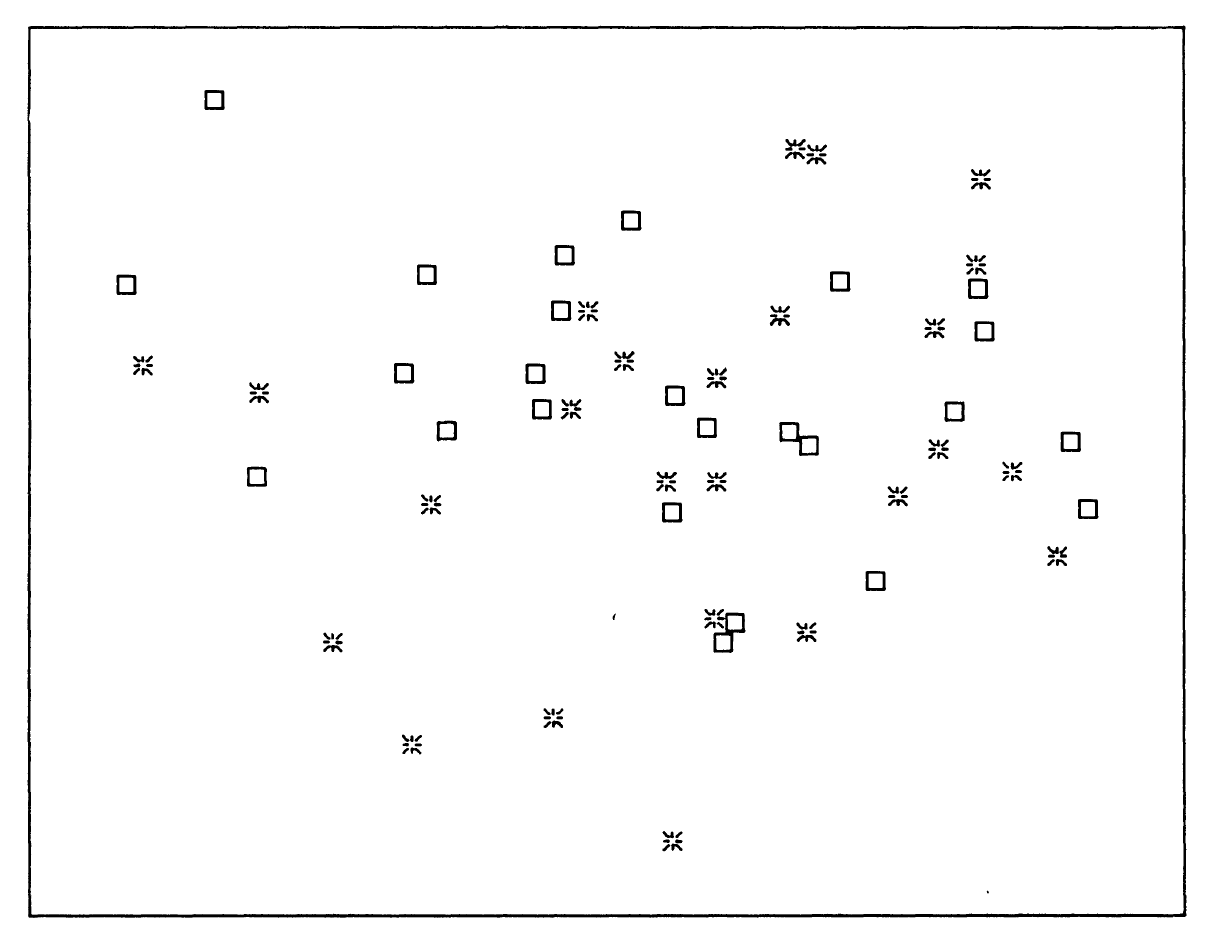
\includegraphics[width=\textwidth]{figure/GCPD_1a.png}
		\caption{original data}\label{fig:GCPD_1a}
	\end{subfigure}
    \begin{subfigure}{.31\textwidth}
		\centering
		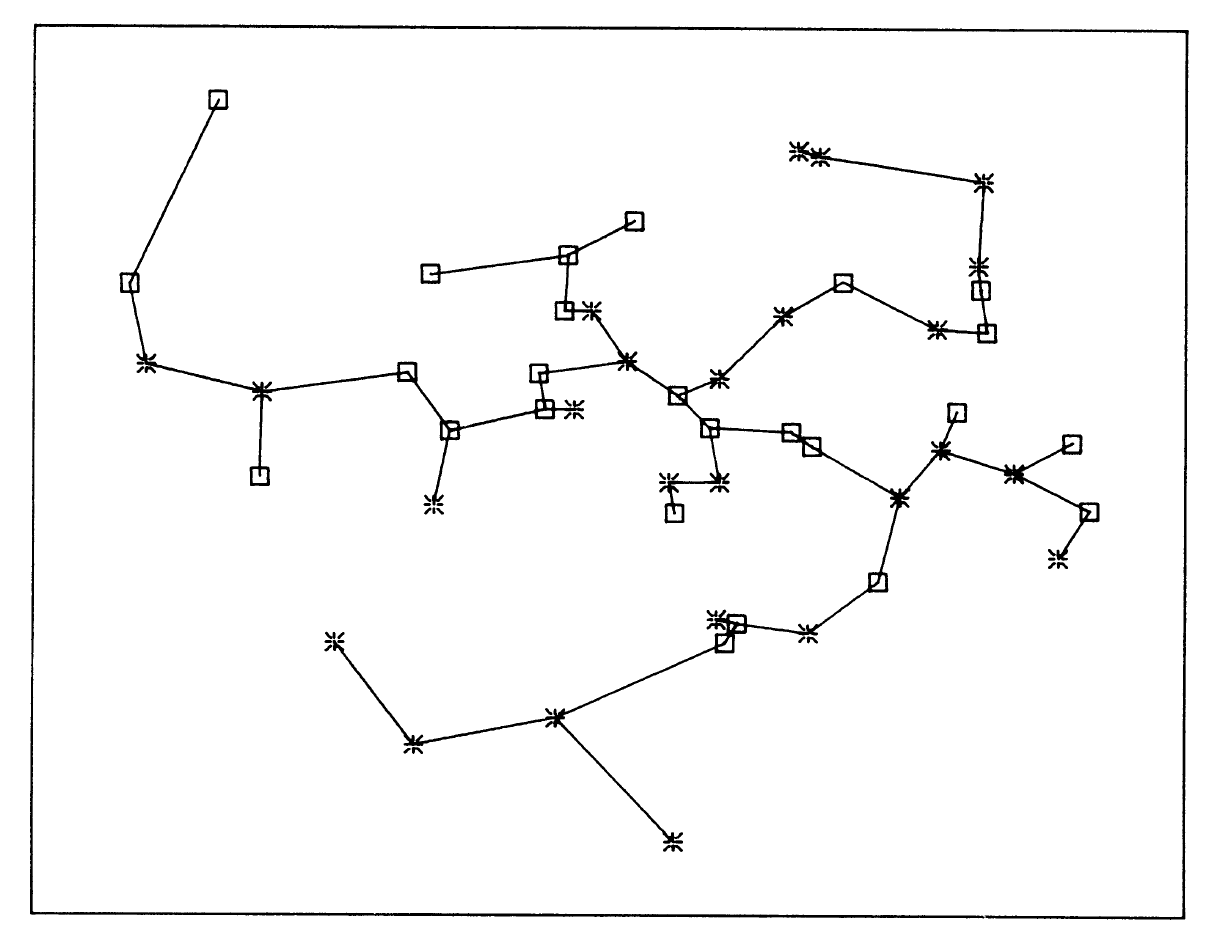
\includegraphics[width=\textwidth]{figure/GCPD_1b.png}
		\caption{MST}\label{fig:GCPD_1b}
	\end{subfigure}
    \begin{subfigure}{.31\textwidth}
		\centering
		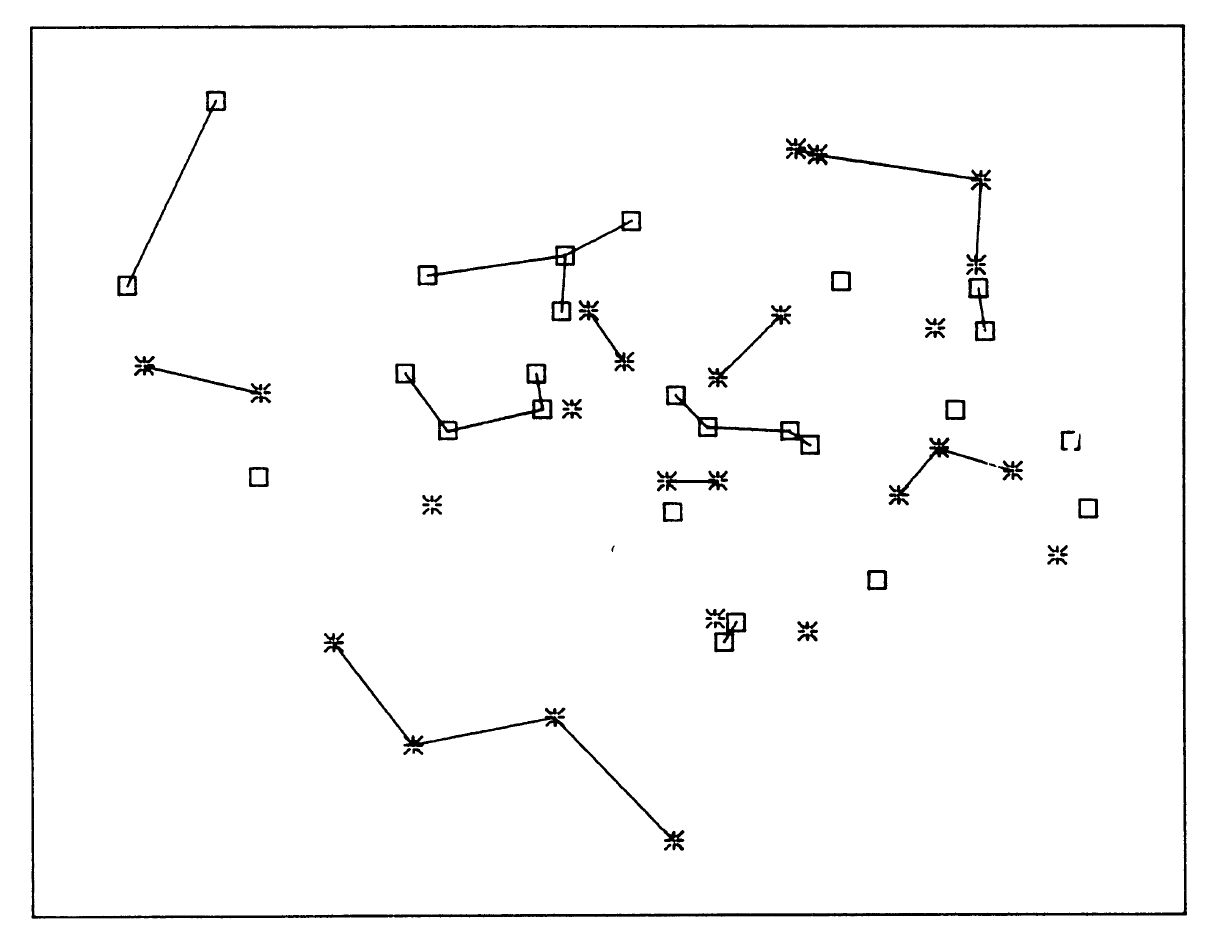
\includegraphics[width=\textwidth]{figure/GCPD_1c.png}
		\caption{remove edges}\label{fig:GCPD_1c}
	\end{subfigure}
    \caption[]{Example of Graph-based method (Friedman et al. 1979)}\label{fig:GCPD_1}
    \end{figure}
\end{frame}

\subsection{Discussion \& Comparison}

\begin{frame}{Discussion}
    \begin{itemize}
        \item Interrupted time series focuses on the impact of sudden events on the entire time series.
        
        \item Change point detection focuses on detecting local points of change within the time series.
        
        \item Both are essential concepts in time series analysis, aiding in understanding and managing uncertainty and variability in data.

        \item Interrupted time series need to know where the trend changes, while change point detection finds these signals. 
    \end{itemize}
\end{frame}

\begin{frame}{Comparison}
    \begin{itemize}
        \item \textbf{Computational cost}\\
        As the dimension of the time series increases, the non-parametric methods will be less expensive than parametric methods\\
        \smallskip
        The cost of supervised methods involved the run time of the training and the CP detection, which is hard to characterize
        \bigskip
        
        \item \textbf{Constraint}\\
        Supervised methods are more accurate than unsupervised ones if there is enough training data and the series is stationary. \\
        \smallskip
        Non-parametric methods are more robust than parametric ones. \\
        \smallskip
        Most unsupervised CPD algorithms operate on limited types of time series data, such as 1-dimensional time series, i.i.d.
    \end{itemize}
\end{frame}

\section[Variance CPD]{Variance Change Point Detection}

\begin{frame}{Variance change point detection}
    \begin{itemize}
        \item The following introduces the variance change point detection method by using the cumulative sum of squares

        \item Let $C_k=\sum_{t=1}^k a_t^2$ be the cumulative sum of squares of a series of uncorrelated random variables $\{ a_t \}$ with mean $0$ and variances $\sigma_t^2, t = 1,2, \cdots, T$. Let
        \begin{align*}
            D_k = \frac{C_k}{C_T}-\frac{k}{T}, \quad k=1,\cdots,T, \quad \mbox{with} \quad D_0=D_T=0
        \end{align*}
         be the centered (and normalized) cumulative sum of squares
    \end{itemize}
\end{frame}

\begin{frame}{Variance change point detection}
    \begin{itemize}
        \item For a fixed $k$, let the first sample be $a_i, i = 1,\cdots,k$, with variance $\tau_0^2$, and let the second sample be $a_j, j = k + 1,...,T$, with variance $\tau_1^2$ \\
        \smallskip
        Then the $F$ statistic for testing $H_0: \tau_0^2 = \tau_1^2$ against $H_a: \tau_0^2 < \tau_1^2$ is $F_{T-k,k} = ((C_T-C_k)/(T-k))/(C_k/k)$ \\
        \smallskip
        Thus, $D_k$ can be expressed in terms of $F_{T-k,k}$ as
        \begin{align*}
            D_k = \frac{C_k}{C_T}-\frac{k}{T} = \frac{k(T-k)}{T^2} \left[\frac{1-F_{T-k,k}}{\frac{k}{T}+\frac{T-k}{T}F_{T-k,k}} \right]
        \end{align*}

        \item we will be looking for $\max_k |D_k|$ to determine the location of the change point
    \end{itemize}
\end{frame}

\begin{frame}{Variance change point detection}
    \begin{figure}
        \centering
        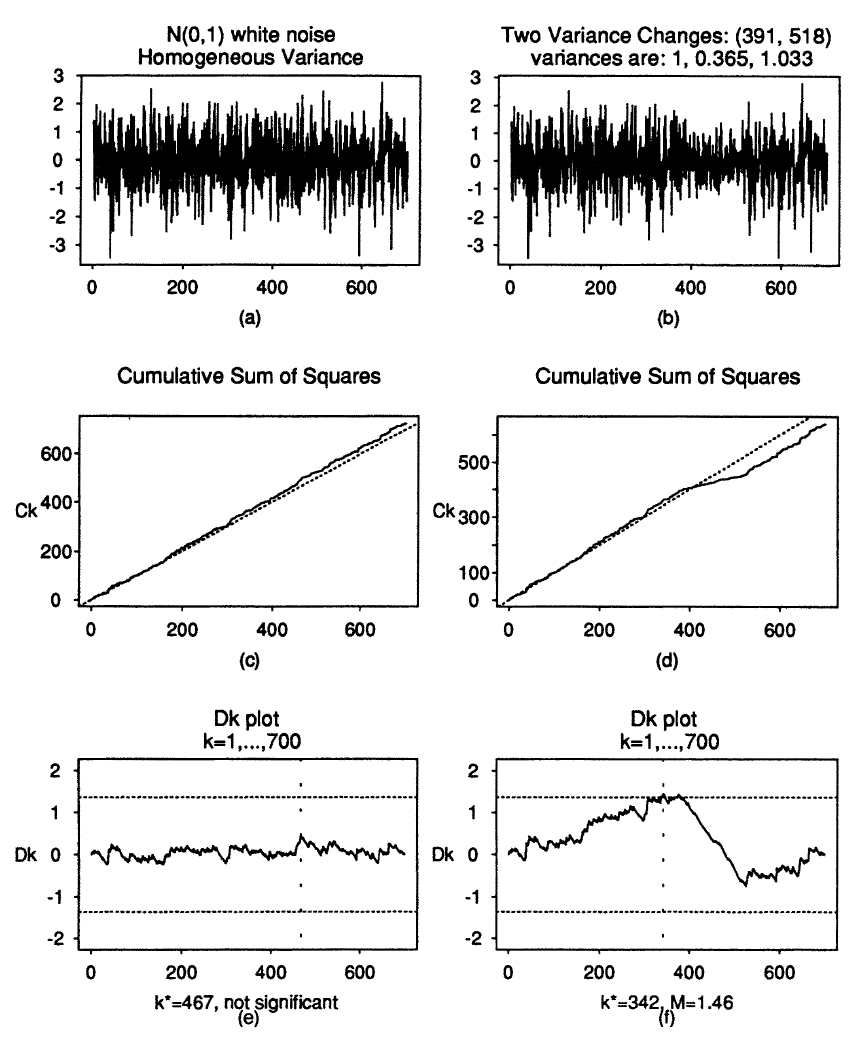
\includegraphics[width=5.5cm]{figure/varCPD.png}
        \caption{Cumulative Sums of Squares Plots (Inclan et al. 1994)}
        \label{fig:varCPD}
    \end{figure}
\end{frame}

\section{Advanced topics}


\subsection{Mixed-frequency data}

\begin{frame}{Mixed-frequency data}
    \begin{itemize}
        %\item Mixed frequency regression model involves time series data sampled at different frequencies.
        
        \item Suppose $\{y_t\}$ is a low frequency variable, whereas $\{x_t^i\}_{i=1}^K$ are at a higher frequency. In particular, for every $1 \leq i \leq K$, there are $m_i$ observations of $x_i$ for a single observation of the response $y$

        \item We want to project the $y_t$ variable onto a history of lagged observations of itself, as well as $\{x_t^i\}_{i=1}^K$
        \begin{align*}
            y_t = \sum_{i=1}^d \alpha_i y_{t-i} + \sum_{i=1}^K \sum_{j=0}^{p_i} \beta_j^i x_{t-j/m_i}^i + \varepsilon_t
        \end{align*}

        \item However, the number of parameters to be estimated can be very large (hundred of indicators or higher frequency), so we need to reduce the effective number of parameters
    \end{itemize}
\end{frame}

\begin{frame}{Mixed-frequency data}
    \begin{itemize}
        \item Ghysels et al. (2007) proposed the use of distributed lag polynomials that involve few parameters and can be estimated using non-linear least squares algorithms

        \item A popular functional form of the polynomial is the exponential Almon lag and Beta Almon lag given by
        \begin{align*}
            \beta_j^i &\propto \frac{\exp(\eta_1^i j + \eta_2^i j^2)}{\sum_{k=0}^{p_i}\exp(\eta_1^i k + \eta_2^i k^2)}\\
            \beta_j^i &\propto \frac{j^{\eta_1^i-1}(p_i+1-j)^{\eta_2^i-1}}{\sum_{k=0}^{p_i} k^{\eta_1^i-1}(p_i+1-k)^{\eta_2^i-1}}
        \end{align*}

        \item Estimation by non-linear least squares and selection of lag through AIC/BIC
    \end{itemize}
\end{frame}

\begin{frame}{Mixed-frequency data}
    \begin{itemize}
        \item Ghosh et al. (2022) develop a Bayesian version of the nested lasso in the context of mixed frequency time series regression
        \bigskip
        
        \item Reparametrize by $\beta_l = \prod_{i=0}^l \theta_i$. Observed that if $\theta_k=0$, then $\beta_j=0, \forall j \geq k$
        \bigskip
        
        \item minimizing an objective function with the penalty $|\beta_1| + \sum_{i=2}^p |\beta_i/\beta_{i-1}|$ will achieve the goal
    \end{itemize}
\end{frame}

\subsection{Multivariate time series}

\begin{frame}{Multivariate time series}
    \begin{itemize}
        \item There are several machine learning (deep learning) approaches that can be employed for analyzing \textbf{multivariate} time series:
        \medskip
        
        \item \textbf{Recurrent Neural Networks (RNNs):} \\
        a type of NN designed to handle sequential data. They can capture dependencies and are suitable for time series.
        
        \item \textbf{Long Short-Term Memory (LSTM):} \\
        a specific type of RNN that is particularly effective in capturing long-term dependencies in time series data
        
        \item \textbf{Gated Recurrent Unit (GRU):} \\
        another variant of RNN that is similar to LSTM but with a simplified structure

        \item \textbf{Temporal Convolution Network (TCN):}\\
        It uses causal and dilated convolutions to capture long-range dependencies efficiently.
    \end{itemize}
\end{frame}


\begin{frame}{Future work}
    \begin{itemize}
        \item Changes in the correlation, distribution
        \bigskip

        \item Multiple change point detection (in multivariate time series)
        \bigskip

        \item Dependent variables and non-stationary time series
        \bigskip

        \item Discussion on scalability and algorithm constraints
    \end{itemize}
\end{frame}

%\section{Reference}

\begin{frame}[allowframebreaks]{Reference}
    \nocite{*}
    \AtNextBibliography{\scriptsize}
    \printbibliography
\end{frame}

\end{document}
